\documentclass{article}

\usepackage[paperwidth=118.9cm,paperheight=84.1cm,margin=1.45cm]{geometry}
\usepackage[T1]{fontenc}
\usepackage{amsmath,amssymb}
\usepackage{array}
\usepackage{booktabs}
\usepackage{graphicx}
\usepackage{xcolor}
\usepackage{enumitem}
\usepackage{helvet}

\renewcommand{\familydefault}{\sfdefault}
\pagestyle{empty}
\setlength{\parindent}{0pt}
\setlength{\parskip}{0.18cm}
\setlist[itemize]{leftmargin=1.05em,itemsep=0.12cm,topsep=0.08cm}
\setlength{\fboxsep}{0.46cm}
\setlength{\fboxrule}{1.1pt}

\definecolor{ink}{HTML}{111827}
\definecolor{muted}{HTML}{475569}
\definecolor{navy}{HTML}{172033}
\definecolor{panel}{HTML}{F8FAFC}
\definecolor{panelwarm}{HTML}{FFF7ED}
\definecolor{line}{HTML}{CBD5E1}
\definecolor{teal}{HTML}{0F766E}
\definecolor{blue}{HTML}{2563EB}
\definecolor{amber}{HTML}{B45309}
\definecolor{green}{HTML}{15803D}
\definecolor{crimson}{HTML}{BE123C}

\newlength{\sepwidth}
\newlength{\colwidth}
\setlength{\sepwidth}{0.022\textwidth}
\setlength{\colwidth}{0.318\textwidth}

\newcommand{\smallcaption}[1]{%
  \vspace{0.08cm}{\fontsize{17}{21}\selectfont\color{muted}#1\par}%
}

\newcommand{\metric}[3]{%
  \begin{minipage}[t]{0.31\linewidth}
    {\fontsize{17}{20}\selectfont\color{muted}#1}\par
    {\fontsize{30}{34}\selectfont\bfseries\color{#3}#2}
  \end{minipage}
}

\newcommand{\plainblock}[2]{%
  \vspace{0.38cm}
  {\fontsize{27}{32}\selectfont\bfseries\color{#2}#1}\par
  \vspace{0.12cm}
}

\begin{document}
\color{ink}
\fontsize{22}{27}\selectfont

\noindent\colorbox{navy}{%
  \begin{minipage}{\dimexpr\textwidth-2\fboxsep\relax}
    \vspace{0.22cm}
    {\fontsize{57}{64}\selectfont\bfseries\color{white}Verifiable Rewards as an Information Bottleneck}\par
    \vspace{0.24cm}
    {\fontsize{27}{33}\selectfont\color{white}One feedback-channel view across self-play, fixed-dataset LLM RLVR, and diffusion-model RL}\par
    \vspace{0.10cm}
    {\fontsize{18}{23}\selectfont\color{white}Poster synthesized from Connect Four, LLM RLVR, and SDXL DDPO modules in \texttt{poster/}.}
    \vspace{0.22cm}
  \end{minipage}
}

\vspace{0.46cm}

\noindent\fcolorbox{line}{panelwarm}{%
  \begin{minipage}{\dimexpr\textwidth-2\fboxsep-2\fboxrule\relax}
    \begin{minipage}[t]{0.31\linewidth}
      {\fontsize{29}{34}\selectfont\bfseries\color{amber}Central claim}\par
      Verifiable rewards reduce evaluator bias, but they compress a rich trajectory into a narrow outcome channel. Learning is strong only when reward variation is aligned with policy-controllable rollout differences.
    \end{minipage}\hfill
    \begin{minipage}[t]{0.35\linewidth}
      \[
        g_\theta(x)
        =
        \operatorname{Cov}_{\tau \sim q_\theta(\cdot\mid x)}
        \left(R(x,\tau),\, \nabla_\theta \log q_\theta(\tau\mid x)\right)
      \]
    \end{minipage}\hfill
    \begin{minipage}[t]{0.28\linewidth}
      {\fontsize{20}{24}\selectfont
      Binary verifier: $\operatorname{Var}[V\mid x]=p(x)(1-p(x))$.\par
      Group signal appears only for mixed rollouts:
      $1-p^K-(1-p)^K$.}
    \end{minipage}
  \end{minipage}
}

\vspace{0.34cm}

\noindent
\begin{minipage}[t]{\colwidth}
  \plainblock{1. Connect Four: self-play renews the channel}{teal}
  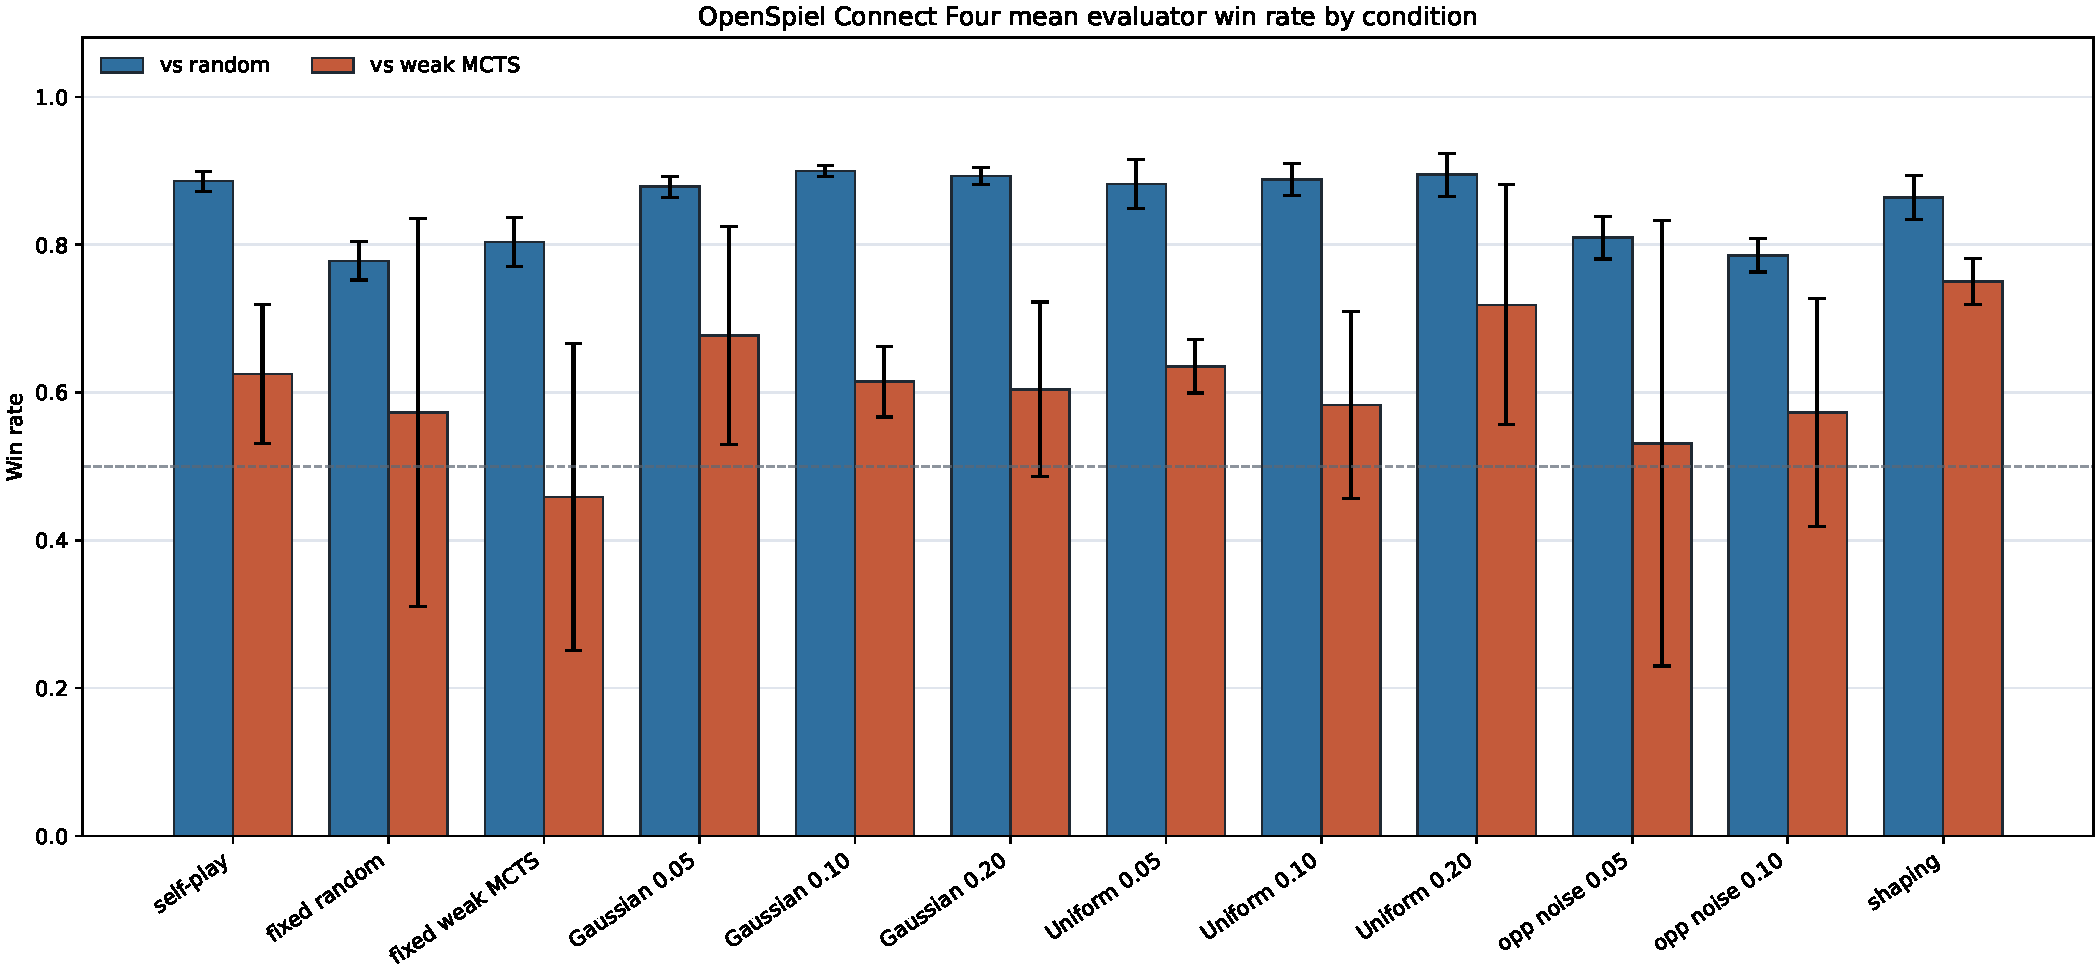
\includegraphics[width=\linewidth,height=13.8cm,keepaspectratio]{connectfour/openspiel_c4_mean_win_rate_by_condition.pdf}
  \smallcaption{OpenSpiel Connect Four evaluation under different training conditions.}

  \begin{itemize}
    \item Self-play keeps the opponent and state distribution near the current policy frontier, so terminal $0/1$ rewards can remain locally informative.
    \item Mean win rates: self-play reaches $0.886$ vs random and $0.625$ vs weak MCTS; fixed-random and fixed-weak opponents produce less reliable generalization.
    \item Larger updates are not the same as useful information: fixed opponents show higher gradient norms, but not better policy quality.
    \item Light process shaping improves weak-MCTS mean win rate from $0.625$ to $0.750$, suggesting that denser feedback can help when it is aligned with contested decisions.
  \end{itemize}

  \vspace{0.25cm}
  \noindent\fcolorbox{line}{panel}{%
    \begin{minipage}{\dimexpr\linewidth-2\fboxsep-2\fboxrule\relax}
      \metric{self-play random win}{0.886}{teal}\hfill
      \metric{self-play weak-MCTS win}{0.625}{teal}\hfill
      \metric{shaped weak-MCTS win}{0.750}{teal}
    \end{minipage}
  }

  \plainblock{Interpretation}{teal}
  AlphaZero-like self-play does not make each reward less sparse. It makes the feedback source renewable: as the policy improves, the task distribution moves with it, keeping many rollouts close to the high-variance decision boundary.
\end{minipage}
\hspace{\sepwidth}
\begin{minipage}[t]{\colwidth}
  \plainblock{2. LLM RLVR: fixed prompts bound verifier information}{blue}
  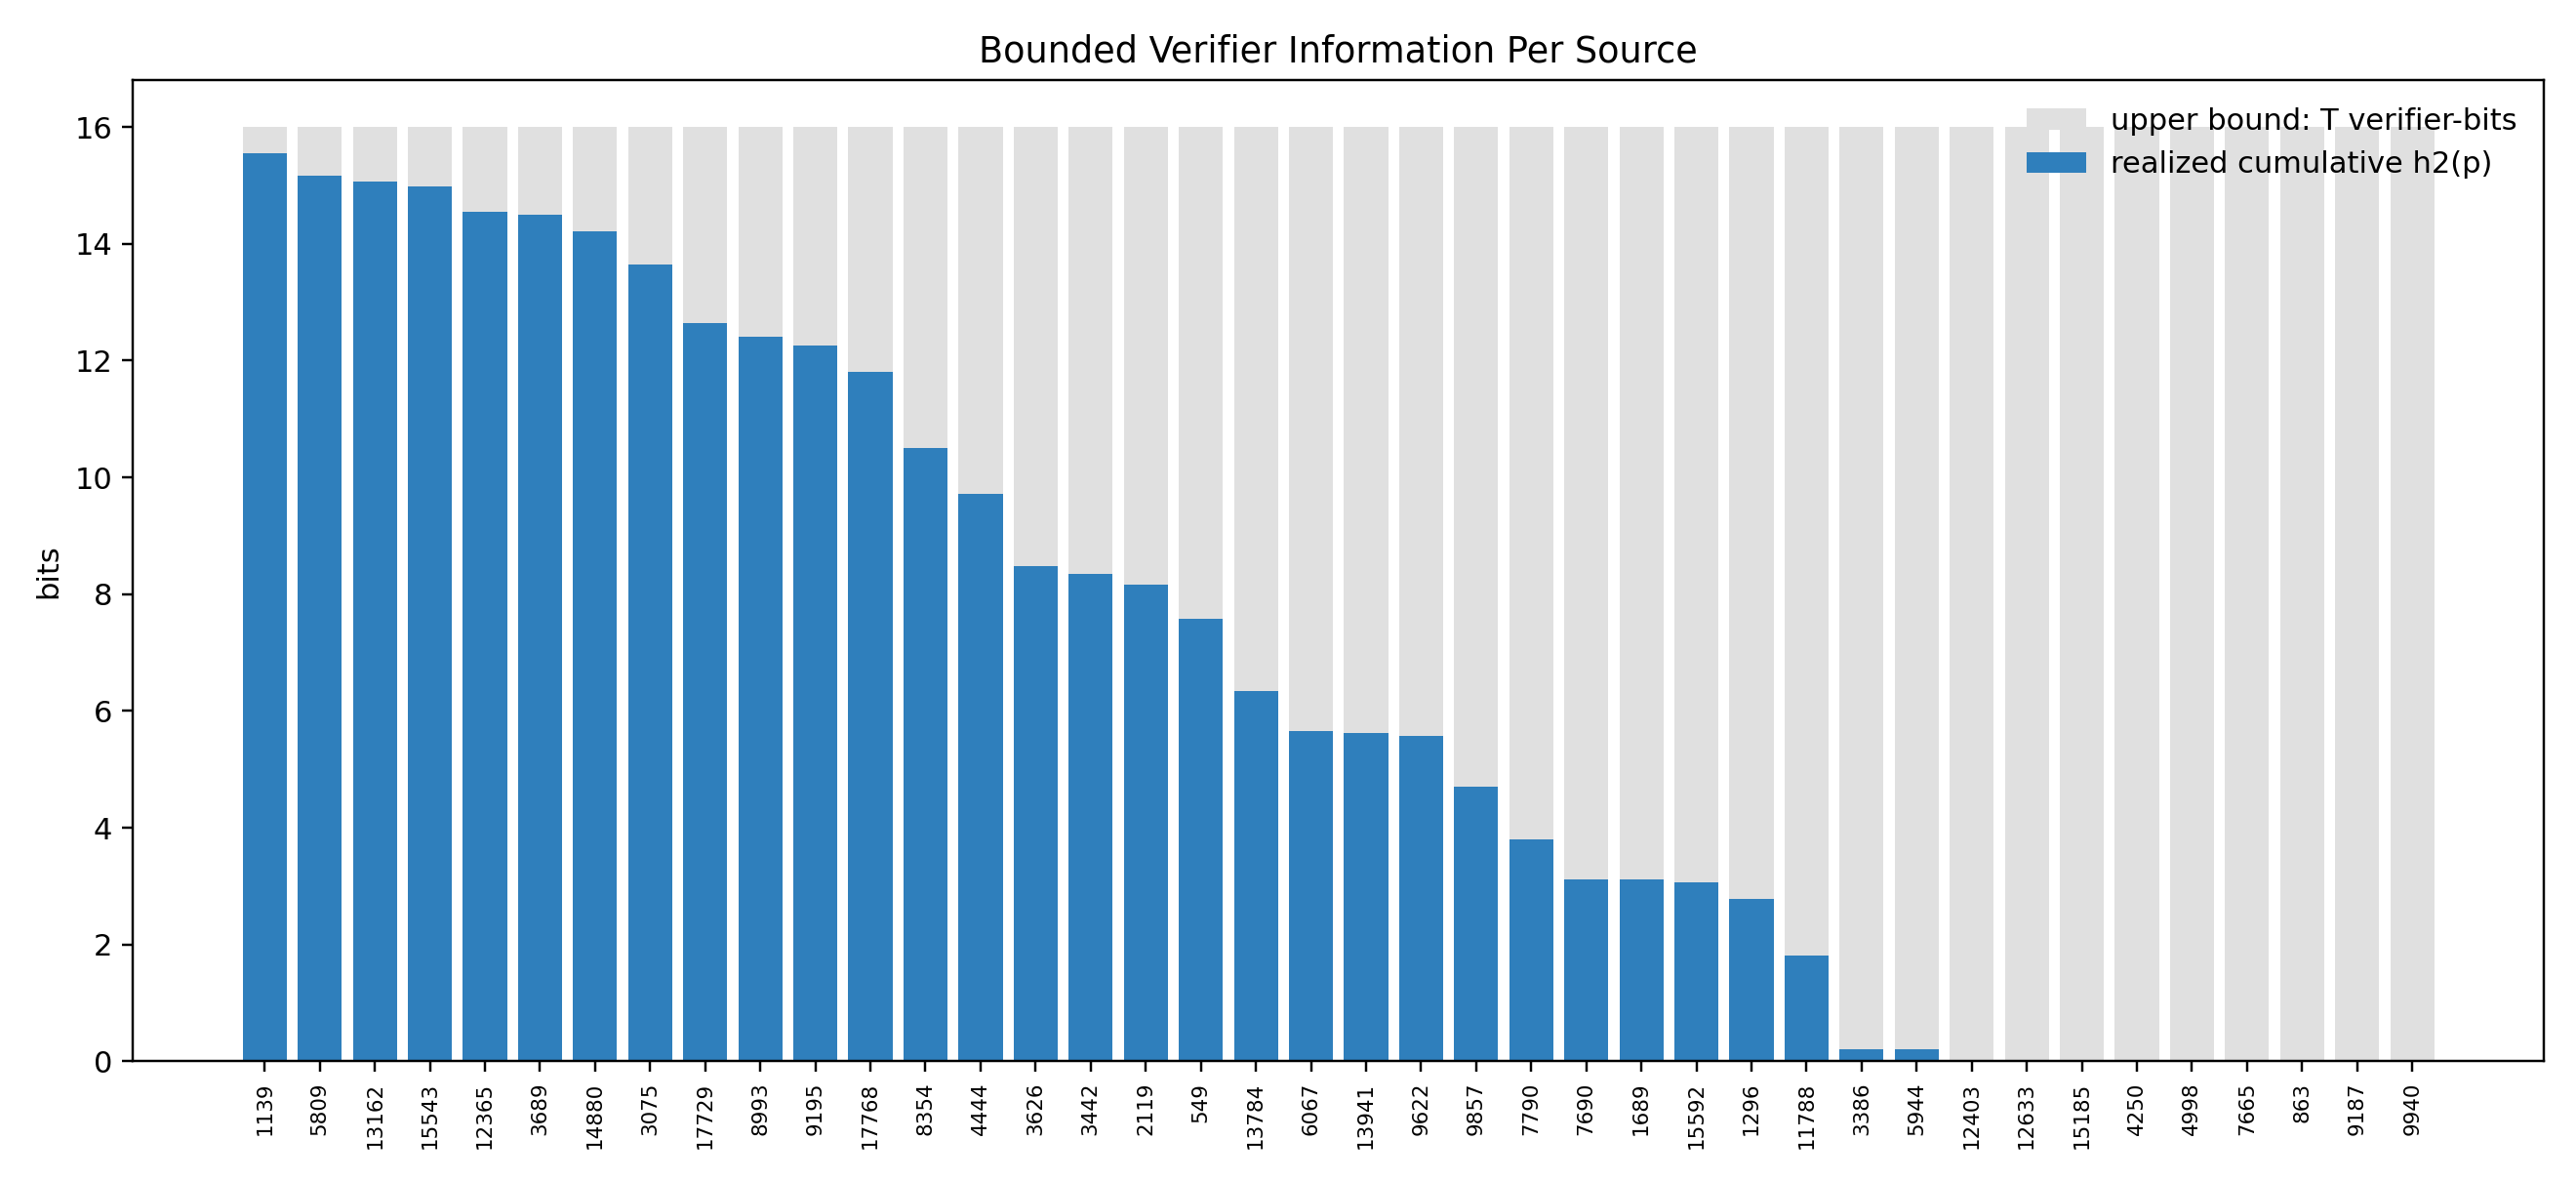
\includegraphics[width=\linewidth,height=12.1cm,keepaspectratio]{llm_rl/assets/figures/geometry40/bounded_information_budget.png}
  \smallcaption{Realized cumulative binary-verifier uncertainty per source prompt in the 40-prompt run.}

  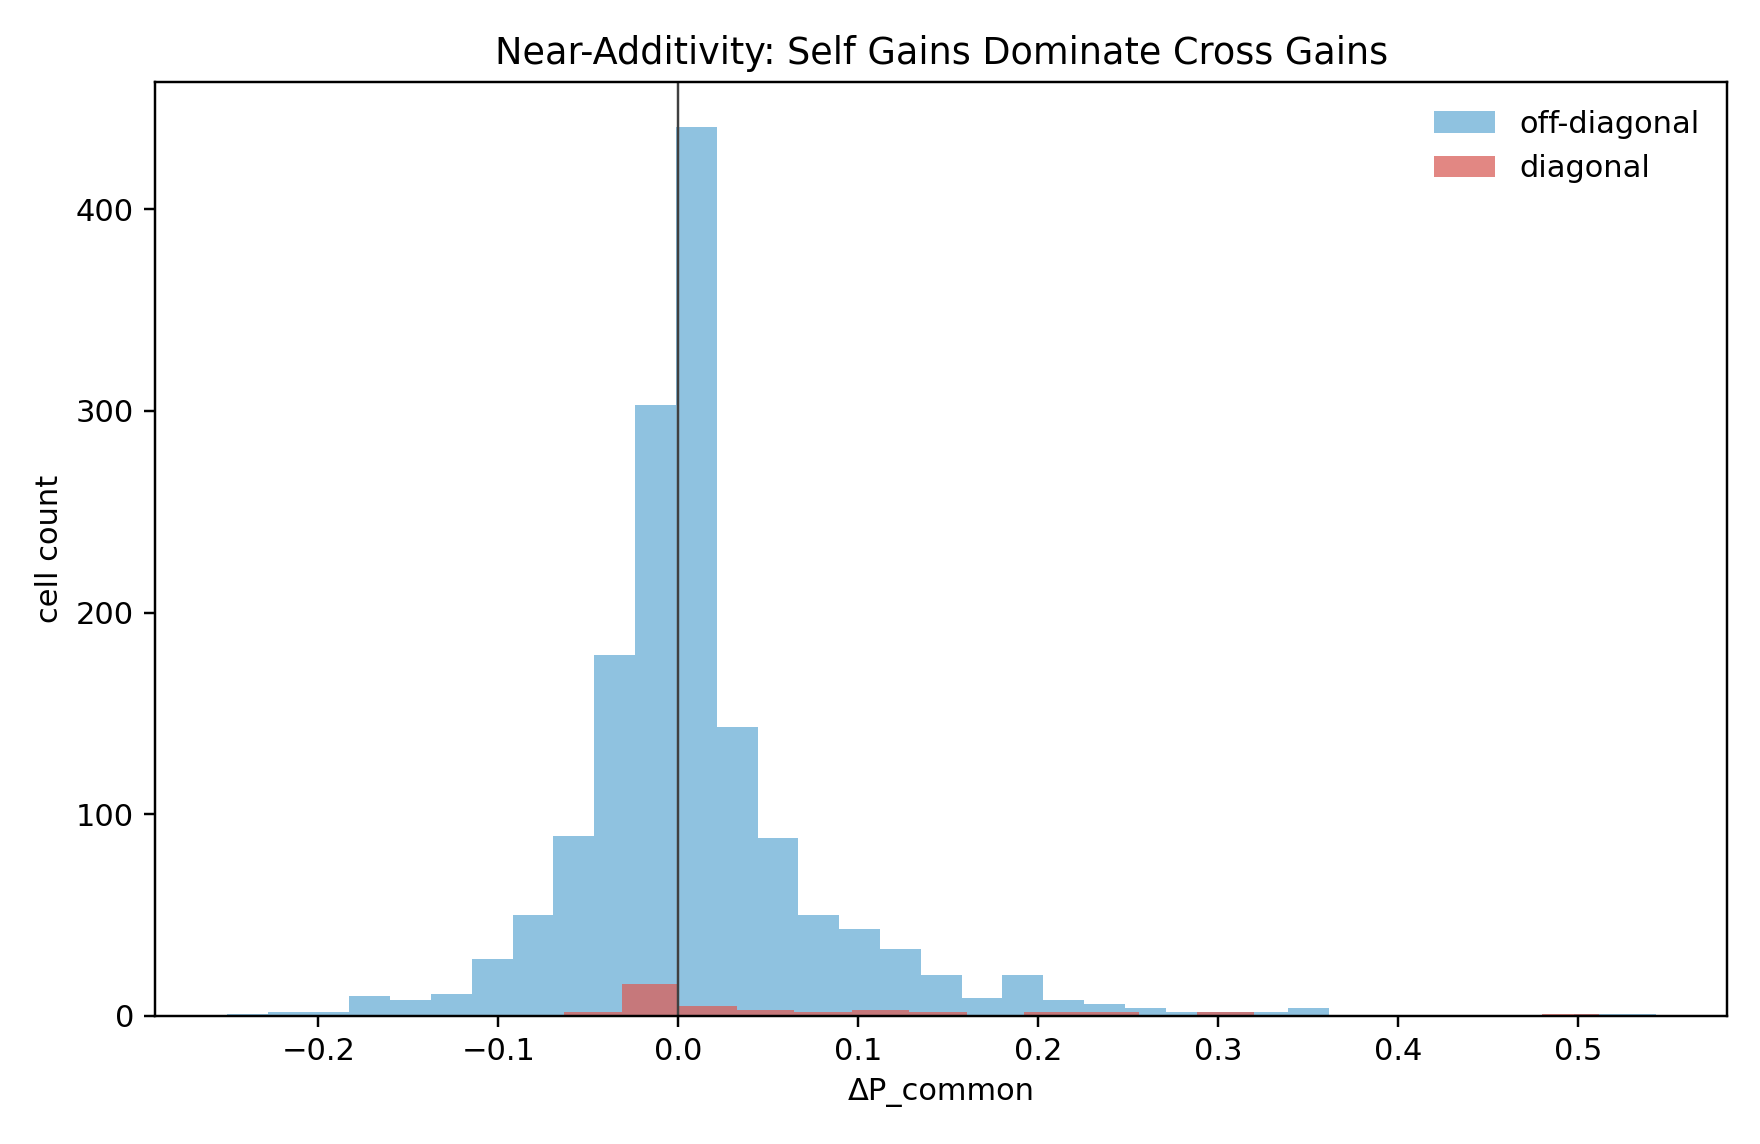
\includegraphics[width=\linewidth,height=11.4cm,keepaspectratio]{llm_rl/assets/figures/geometry40/diag_vs_offdiag_transfer_histogram.png}
  \smallcaption{Endpoint transfer: self gains dominate sparse cross-prompt gains.}

  \begin{itemize}
    \item A fixed verifier dataset has a finite per-step binary budget: $H_i(t)=h_2(p_i(t))\le 1$ bit.
    \item In the 40-prompt run, realized verifier uncertainty is $265.5/640.0$ step-bits, or $41.5\%$ of the simple upper bound.
    \item Self-transfer dominates cross-transfer: mean diagonal $\Delta P=0.0706$, mean off-diagonal $\Delta P=0.0091$, ratio $0.129$, additivity score $0.871$.
    \item RLVR also shrinks rollout action distributions: correct-only entropy changes from $0.217$ to $0.202$ nats/token.
  \end{itemize}

  \vspace{0.25cm}
  \noindent\fcolorbox{line}{panel}{%
    \begin{minipage}{\dimexpr\linewidth-2\fboxsep-2\fboxrule\relax}
      \metric{used verifier budget}{41.5\%}{blue}\hfill
      \metric{offdiag / diag}{0.129}{blue}\hfill
      \metric{2D transfer variance}{48.3\%}{blue}
    \end{minipage}
  }

  \plainblock{Interpretation}{blue}
  Fixed-dataset RLVR is bottlenecked by prompts that are too easy, too hard, or sampled with zero within-group reward variance. Cross-prompt transfer exists, but most useful mass remains prompt-local unless allocation or curriculum mechanisms refresh the frontier.
\end{minipage}
\hspace{\sepwidth}
\begin{minipage}[t]{\colwidth}
  \plainblock{3. Diffusion RL: richer channels help, alignment still matters}{green}
  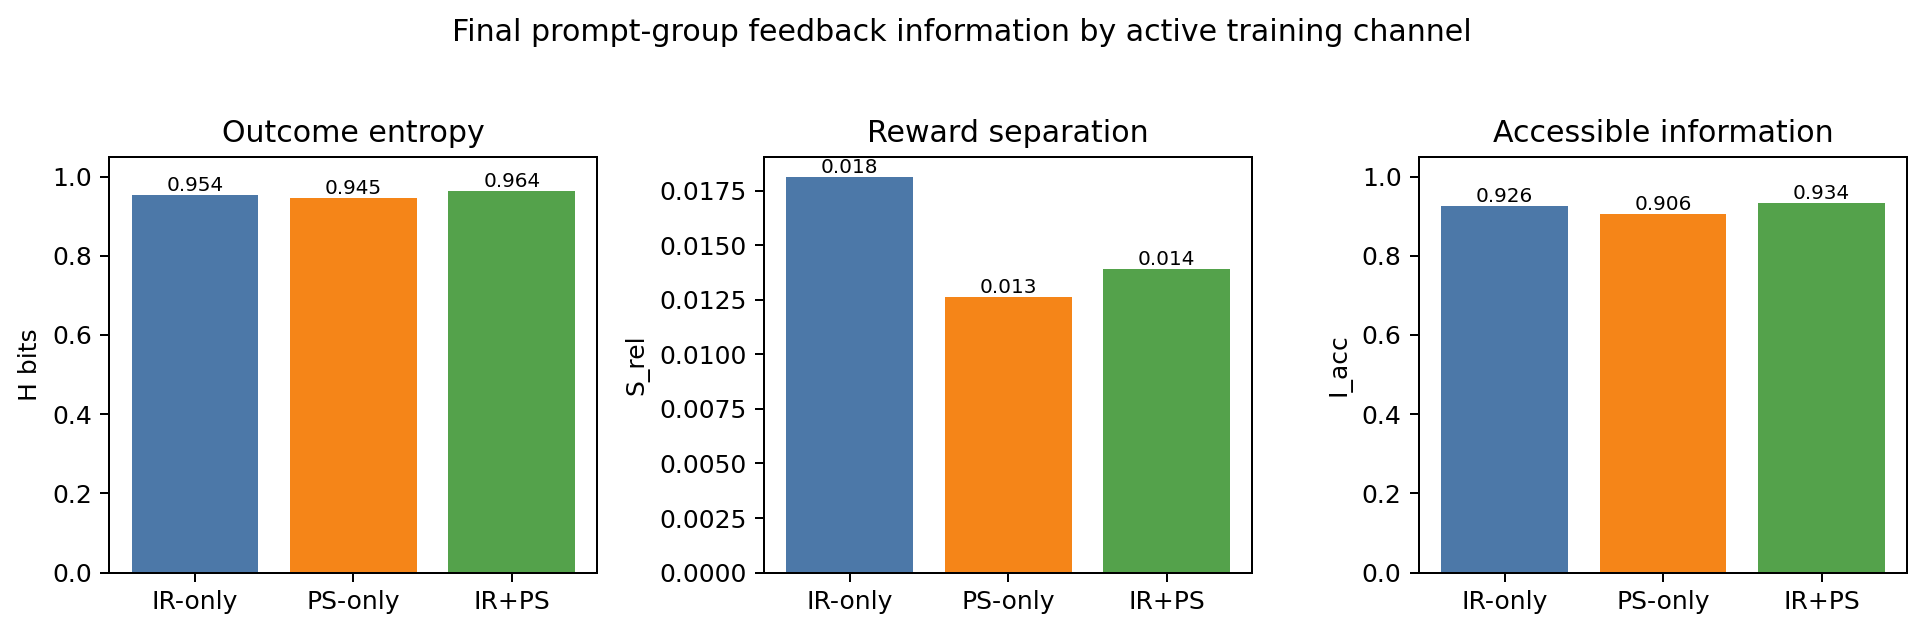
\includegraphics[width=\linewidth,height=10.0cm,keepaspectratio]{diffusion_rl/figures/information_bottleneck/final_active_channel_information.png}
  \smallcaption{Prompt-group feedback information for active SDXL DDPO training channels.}

  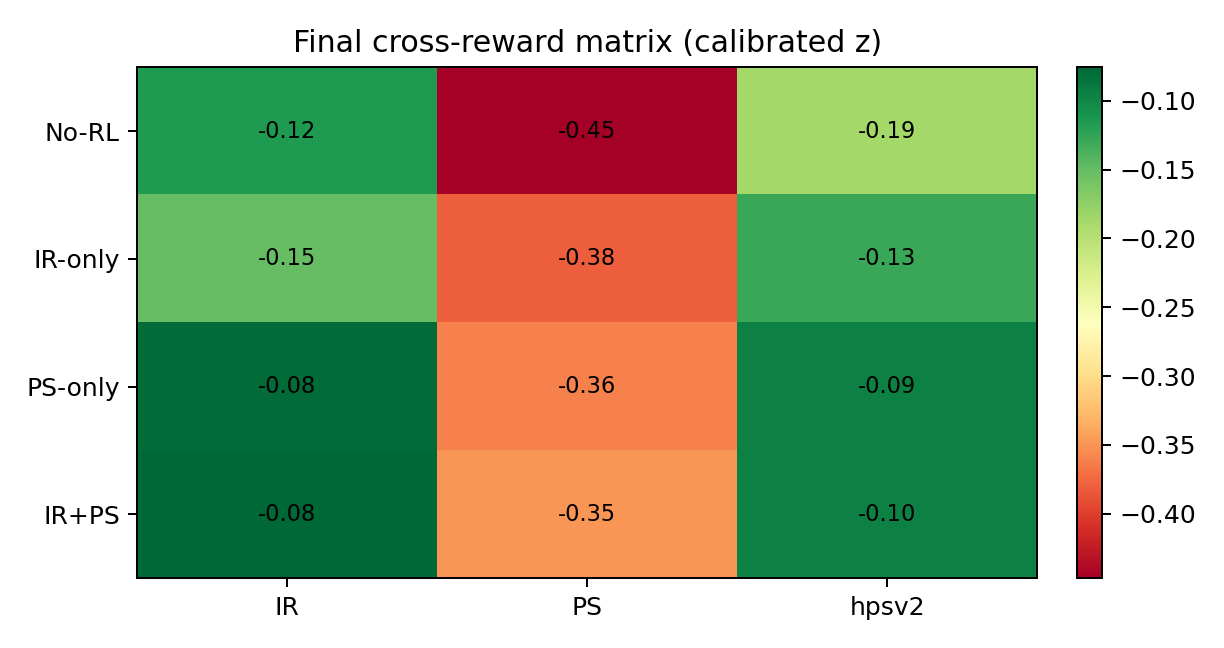
\includegraphics[width=\linewidth,height=12.5cm,keepaspectratio]{diffusion_rl/figures/main/cross_reward_matrix_final_z.png}
  \smallcaption{Final cross-reward matrix over ImageReward, PickScore, and held-out HPSv2.}

  \begin{itemize}
    \item One-prompt DDPO was unstable: base quality and reward mismatch dominated the result.
    \item With 10 prompt-balanced prompts, all RL conditions improve final held-out HPSv2 over No-RL.
    \item Active-channel accessible information is highest for the hybrid IR+PS channel: $I_{\mathrm{acc}}=0.934$.
    \item IR+PS is best on ImageReward and PickScore and nearly ties PS-only on HPSv2; this separates feedback richness from evaluator alignment.
  \end{itemize}

  \vspace{0.25cm}
  \noindent\fcolorbox{line}{panel}{%
    \begin{minipage}{\dimexpr\linewidth-2\fboxsep-2\fboxrule\relax}
      \metric{IR+PS active $I_{\rm acc}$}{0.934}{green}\hfill
      \metric{PS-only HPSv2 z}{-0.0947}{green}\hfill
      \metric{IR+PS HPSv2 z}{-0.0958}{green}
    \end{minipage}
  }

  \plainblock{Interpretation}{green}
  Diffusion rewards are graded rather than binary, but the same bottleneck appears at the prompt-group level. Reward models must distinguish multiple images for the same prompt, and the informative channel must also align with the held-out evaluator.
\end{minipage}

\vspace{0.50cm}

\noindent\fcolorbox{line}{panel}{%
  \begin{minipage}{\dimexpr\textwidth-2\fboxsep-2\fboxrule\relax}
    {\fontsize{29}{34}\selectfont\bfseries\color{crimson}Unified picture and design implications}\par
    \vspace{0.18cm}
    \begin{minipage}[t]{0.31\linewidth}
      {\fontsize{23}{28}\selectfont\bfseries Renew the frontier}\par
      Self-play keeps terminal rewards useful by continuously generating contested trajectories. Fixed datasets need curricula, new prompts, adaptive sampling, or self-generated variants to avoid verifier-information depletion.
    \end{minipage}\hfill
    \begin{minipage}[t]{0.31\linewidth}
      {\fontsize{23}{28}\selectfont\bfseries Allocate verifier queries}\par
      Spend rollout budget where $p(1-p)$ and mixed-group probability are high. Avoid all-correct and all-wrong groups unless exploration or dense feedback can recover contrast.
    \end{minipage}\hfill
    \begin{minipage}[t]{0.31\linewidth}
      {\fontsize{23}{28}\selectfont\bfseries Enrich without misaligning}\par
      Dense, process, or multi-reward channels can expose more distinctions among rollouts, but final performance still depends on whether those distinctions match the target task or evaluator.
    \end{minipage}
  \end{minipage}
}

\vfill
{\fontsize{15}{18}\selectfont\color{muted}
Template choice: a Gemini/beamerposter-inspired three-column research-poster layout, implemented as a self-contained \LaTeX{} article for local \texttt{tectonic} compilation. Figures are selected from \texttt{poster/connectfour}, \texttt{poster/llm\_rl}, and \texttt{poster/diffusion\_rl}.}

\end{document}
